%\documentclass[11pt,a4paper]{scrartcl}
\documentclass{MSM_latex}
\author{M. Denkinger, S. Eyes, J. Schnitzler}


\makeatletter
\let\runauthor\@author
\let\rundate\@date
% Fußzeile
\lfoot{\textit{\runauthor} \\ \textit{\rundate}}
%%%%%%%%%%%%%%%%%%%%%%%%%%%%%%%%%%%%%%%%%%%%%%%%%%%5
% Matlab-Code
\usepackage{listings}
\usepackage{color}

\definecolor{mygreen}{rgb}{0,0.6,0}
\definecolor{mygray}{rgb}{0.5,0.5,0.5}
\definecolor{mymauve}{rgb}{0.58,0,0.82}

\lstset{ %
  backgroundcolor=\color{white},   % choose the background color
  basicstyle=\footnotesize,        % size of fonts used for the code
  breaklines=true,                 % automatic line breaking only at whitespace
  captionpos=b,                    % sets the caption-position to bottom
  commentstyle=\color{mygreen},    % comment style
  escapeinside={\%*}{*)},          % if you want to add LaTeX within your code
  keywordstyle=\color{blue},       % keyword style
  stringstyle=\color{mymauve},     % string literal style
  language=Matlab,                 % the language of the code
  numbers=left,                    % where to put the line-numbers; possible values are (none, left, right)
  numbersep=5pt,                   % how far the line-numbers are from the code
  numberstyle=\tiny\color{mygray}, % line-number style
  rulecolor=\color{black},         % if not set, the frame-color may be changed on line-breaks within not-black text
  showspaces=false,                % show spaces everywhere adding particular underscores; it overrides 'showstringspaces'
  showstringspaces=false,          % underline spaces within string literals
  showtabs=false,                  % show tabs within string literals adding particular underscores
  stepnumber=2,                    % the step between two line-numbers. If it's 1, each line will be numbered
  tabsize=2,                       % sets default tabsize to 2 spaces
  title=\lstname                   % show the filename of files included with \lstinputlisting; also try caption instead of title
  %%%%%%%%%%%%%%%%%%%%%%%%%%%%%%%%%%%%%%%%%%%%%%%%%%%%%%%%%%%%%%%%%%%%%%%


}


\begin{document}


\section{Weihnachtsprojekt: Simulation und Regelung eines Knickarmroboters}

\subsection*{Aufgabe 1 - Bestimmung der Kinematik und DH-Parameter}

Zur Bestimmung der Kinematik ist es notwendig herauszufinden, wie die einzelnen Gelenke des Roboters miteinander verbunden sind.
Die Denavit-Hartenberg-Notation wird verwendet, um die 3D-Transformation zum nächsten Gelenk mithilfe von vier Parameter zu beschreiben. Im Fall des Knickarmroboters ist
dies sehr einfach, da es sich lediglich um eine Kette von drei Gelenken handelt. Die Koordinatentransformation ist jeweils eine Rotation um die $z$-Achse mit $\theta_i$
und eine Translation in der $xy$-Ebene, um die Länge $a_i = l_i$. Wir können somit das erste Gelenk in den Ursprung legen und mithilfe von zwei Transformationen $T_{12}$ und $T_{23}$ alles beschreiben. Um mit einem nicht gedrehten Koordinatensystem anzufangen, benötigen wir zusätzlich $T_{01}$. Die DH-Parameter sind in Tabelle \ref{tab:DH} aufgeführt.



\begin{table}[tb]
	\centering
	\begin{tabular}{lccccr}
		\toprule
		Achse & $a_{i-1}$ & $\alpha_{i-1}$ & $d_i$ & $\theta_i$ & Art \\
		\midrule
		1 & 0& 0& 0& $-90^\circ $& Rotation \\
		2 & $l_1 = 0.16 \text{ m}$& 0& 0& $\alpha$& Translation\\
		3 & $l_2 = 0.128 \text{ m}$& 0& 0& $\beta$& Both\\ 
		\bottomrule
	\end{tabular}
	\caption{DH-Parameter des Knickarmroboters}
	\label{tab:DH}
\end{table}

Daraus resultieren die Transformationsmatrizen
\begin{equation*}
	T_{12}(\alpha, l_1) = \begin{pmatrix}
	\cos(\alpha) & -\sin(\alpha) & 0 & 0 \\
	\sin(\alpha) & \cos(\alpha) & 0 & 0 \\
	0 & 0 & 1 & 0 \\
	0 & 0 & 0 & 1
	\end{pmatrix} \cdot \begin{pmatrix}
	1 & 0 & 0 & l_1 \\
	0 & 1 & 0 & 0 \\
	0 & 0 & 1 & 0 \\
	0 & 0 & 0 & 1
	\end{pmatrix} = \begin{pmatrix}
	\cos(\alpha) & -\sin(\alpha) & 0 & \cos(\alpha) l_1 \\
	\sin(\alpha) & \cos(\alpha) & 0 & \sin(\alpha) l_1 \\
	0 & 0 & 1 & 0 \\
	0 & 0 & 0 & 1
	\end{pmatrix}
\end{equation*}
und
\begin{equation*}
	T_{23}(\beta, l_2) = \begin{pmatrix}
	\cos(\beta) & -\sin(\beta) & 0 & 0 \\
	\sin(\beta) & \cos(\beta) & 0 & 0 \\
	0 & 0 & 1 & 0 \\
	0 & 0 & 0 & 1
	\end{pmatrix} \cdot \begin{pmatrix}
	1 & 0 & 0 & l_2 \\
	0 & 1 & 0 & 0 \\
	0 & 0 & 1 & 0 \\
	0 & 0 & 0 & 1
	\end{pmatrix} = \begin{pmatrix}
	\cos(\beta) & -\sin(\beta) & 0 & \cos(\beta) l_2 \\
	\sin(\beta) & \cos(\beta) & 0 & \sin(\beta) l_2 \\
	0 & 0 & 1 & 0 \\
	0 & 0 & 0 & 1
	\end{pmatrix}
\end{equation*}

Die Gesamttransformation ergibt sich aus der Multiplikation der beiden Matrizen, welche mithilfe von trigonometrischen Additionstheoremen vereinfacht werden kann.

\begin{equation*}
	T_{13} = T_{12} \cdot T_{23} = \begin{pmatrix}
	\cos(\alpha + \beta) & -\sin(\alpha + \beta) & 0 & \cos(\alpha) l_1 + \cos(\alpha + \beta) l_2\\
	\sin(\alpha + \beta) & \cos(\alpha + \beta) & 0 & \sin(\alpha) l_1 + \sin(\alpha + \beta) l_2 \\
	0 & 0 & 1 & 0 \\
	0 & 0 & 0 & 1
	\end{pmatrix}
\end{equation*}

\begin{equation*}
	T_{03} = \begin{pmatrix}
	\cos(\alpha + \beta) & -\sin(\alpha + \beta) & 0 & \cos(\alpha) l_1 + \cos(\alpha + \beta) l_2\\
	\sin(\alpha + \beta) & \cos(\alpha + \beta) & 0 & \sin(\alpha) l_1 + \sin(\alpha + \beta) l_2 \\
	0 & 0 & 1 & 0 \\
	0 & 0 & 0 & 1
	\end{pmatrix}
\end{equation*}

Somit ergibt sich die Position von Gelenk 2 im Weltkoordinatensystem zu
\begin{equation*}
	\begin{pmatrix} x_2 \\ y_2 \\ z_2 \end{pmatrix} = \begin{pmatrix}
	\cos(\alpha) l_1\\ \sin(\alpha) l_1 \\ z_2 \end{pmatrix}
\end{equation*}
und die Position von Gelenk 3 bzw. des Endeffektors zu
\begin{equation*}
	\begin{pmatrix} x_3 \\ y_3 \\ z_3 \end{pmatrix} = 
	\begin{pmatrix}
	\cos(\alpha) l_1 + \cos(\alpha + \beta) l_2\\ \sin(\alpha) l_1 + \sin(\alpha + \beta) l_2 \\ z_3 
	\end{pmatrix}
\end{equation*}

\textit{Anmerkung}: Da die Parameter $\alpha_{i-1}$ und $d_i$ sind immer null sind, ist eine 2D Betrachtung ausreichend, wie man auch an der \emph{Identitäts-Zeile-Spalte} für $z$ erkennen kann.

\subsection*{Aufgabe 2 - Bestimmung der Bewegungsgleichung}

\subsubsection*{Generalisierte Koordinaten}
Die Wahl fällt zu $y(1) = \alpha$ und $y(2) = \beta$. 
Die generalisierten Koordinaten sind somit die Winkel der Gelenke 1 und 2.

\subsubsection*{Lagrang'sche Gleichung 2. Art}
Die Bewegungsgleichung des Arms kann mit folgender Gleichung beschrieben werden:

\begin{equation}
	M(y) \cdot \ddot{y} + D(y,\dot{y}) \cdot \dot{y} + g(y) = \tau_{Reib} + \tau_{Aktormoment}
\end{equation}

Dabei berechnet sich die Massenmatrix $M_{i}$ mit $M = \sum_{i}{M_{i}}$ von Arm i nach:
\begin{equation}
	M_{i}(y) = \left[m_{i}J_{TiS}^{T}(y) \cdot J_{TiS}(y) + 
	J_{RiS}^{T}(y) \cdot S_{0,iS}(y) \cdot I_{iS,iS} \cdot S_{0,is}^{T}(y) J_{RiS}(y) \right]
\end{equation}

Dabei sind $J_{TiS}(y)$ und $J_{RiS}(y)$ die Jakobimatrizen für den Schwerpunkt für Körper 
i der Translation beziehungsweise Rotation und $I_{iS,iS}$
der Trägheitstensor von Körper i dargestellt in dessen Schwerpunkt.

Mithilfe der Transformationsmatrix $S_{0,iS}(y)$ kann der Trägheitstensor im Inertialsystem dargestellt werden:
\begin{equation}
	I_{iS,0} = S_{0,iS}(y) \cdot I_{iS,iS} \cdot S_{0,is}^{T}(y)
\end{equation}


Für  $D(y,\dot{y})$ gilt:
\begin{equation}
	D_{kj} = \sum_{i=1}^{n}h_{ijk}(y)\dot{y}_{i}
\end{equation}
mit den Christoffel-Symbolen
\begin{equation}
	h_{ijk} = \frac{1}{2}\left(	\frac{\partial M_{kj}}{\partial y_{i}} + 
								\frac{\partial M_{ki}}{\partial y_{j }} -
								\frac{\partial M_{ij}}{\partial y_{k}}				\right)
\end{equation}

Der Graviationsvektor $g(y)$ ist definiert als
\begin{equation}
	g(y) = \left[ 
			\frac{\partial{V}}{\partial{y_{1}}} , 
			\frac{\partial{V}}{\partial{y_{2}}}
	\right]^{T}
\end{equation}

mit der potentiellen Energie $V$:
\begin{equation}
	V(y) = \sum_{i}V_{i} = \sum_{i}m_{i}g \cdot p_{iS,0}(y) 
\end{equation}
nach 2.1.11 Lagrange'sche Gleichungen zweiter Art in \cite{Fehr23}.
Die Umsetzung der genannten Gleichungen wurde mit der Symbolic Math Toolbox in Matlab implementiert.
Gleichung (1) liefert dann jeweils eine Differentialgeichung pro generalisierte Koordinate $y_{i}$.



\subsubsection*{Reibungsterm}
In Gleichung (1) geht das Reibmoment der Lagerung der Arme $\tau_{Reib}$ mit ein, welches aus der Überlagerung der viskosen mit der 
statischen Reibung modelliert wird:

\begin{figure}[H]
	\centering
	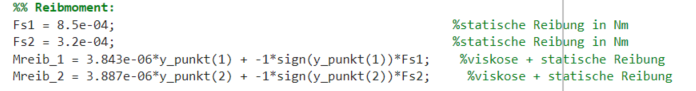
\includegraphics[width=0.95\textwidth]{Reibung.png}
	\caption{Modellierung der Lagerreibung}
\end{figure}



\newpage

\subsection*{Aufgabe 4 - Bewegungsgleichung in Matlab}

Unsere Gruppe hat sich dafür entschieden die Bewegungsgleichung und ihre Lösung direkt in MatLab zu implementieren. Wie bereits in A2 erläutert wurde, haben wir die Symbolic Toolbox von Matlab benutzt, um die Bewegungsgleichung aufzustellen.

Unser Ziel ist es nun gewesen die aufgestellte Ordinary Differential Equations (ODE) mithilfe eines Solvers wie Euler-Vorwärts zu lösen. Dafür haben wir die Funktion \texttt{ode45} benutzt, welche die ODE numerisch löst. Die Funktion \texttt{ode45} benötigt als Eingabe die ODE, die Anfangsbedingungen und den Zeitbereich, in dem die ODE gelöst werden soll. Als Ausgabe liefert die Funktion die Lösung der ODE in Form von Vektoren für die Zeit und die Lösung der ODE. 

Wie vorgegeben haben wir als Optionen des Solvers \texttt{ode45} die \texttt{RelTol} auf $10^{-4}$ und \texttt{AbsTol} auf $10^{-7}$ gesetzt. Die \texttt{RelTol} gibt die relative Toleranz an, die die Lösung der ODE haben darf. Die \texttt{AbsTol} gibt die absolute Toleranz an, die die Lösung der ODE haben darf. Die Toleranzen sind wichtig, da die Lösung der ODE numerisch berechnet wird und somit nicht exakt ist. Die Toleranzen geben an, wie genau die Lösung der ODE sein muss. Außerdem haben wir eine maximale Schrittweite gesetzt mithilfe von \texttt{MaxStep} $=3\cdot 10^{-3}$. 

\subsubsection[short]{Aufstellen der rechten Seite}

Nun benötigen wir noch eine rechte Seite

\begin{lstlisting}[caption={Aufruf der Funktion \texttt{ode45}},label={lst:ode45}]
    % Syntax: y_0 = [alpha; alpha_dot; beta; beta_dot, err_alpha, err_beta]
    y_0 = [pi/2; 0.5; -pi/5; -0.1; 0; 0];
    tspan = [0, 1];
    opts = odeset('RelTol', 1e-4, ...
          'AbsTol', 1e-7, ...
          'MaxStep', 3*1e3);
    
    [t, y] = ode45(odefun, tspan, y0, opts);
\end{lstlisting}




\subsection*{Resultat und Visualisierung}

Animiert wird die Bewegung des Knickarmroboters mithilfe des \texttt{plot} Befehls. Hierfür werden die bereits in Aufgabe 1 erläuterten homogenen Transformationsmatrizen genutzt, um die generalisierten Koordinaten $\alpha$ und $\beta$ auf kartesische Koordinaten zu übersetzen. Das erste Gelenk 

\begin{figure}[H]
    \centering
    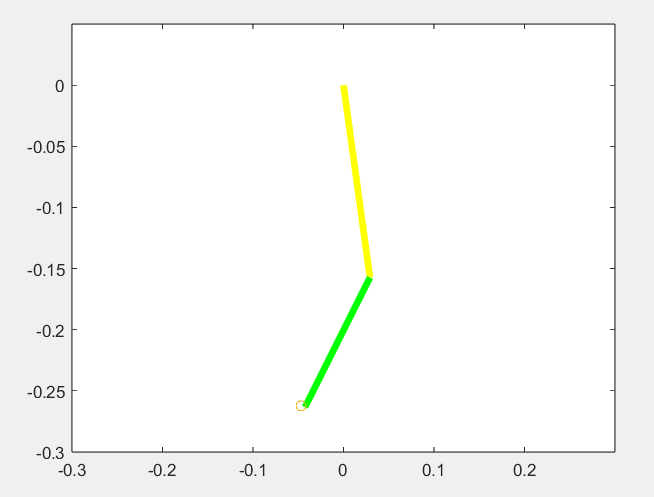
\includegraphics[width=0.8\linewidth]{img/visualisierung.png}
    \caption{Visualisierung der Simulation}
    \label{fig:visualisierung}
\end{figure}


\begin{lstlisting}[caption={Definition der rechten Seite},label={lst:wrapper}]
    %% Visualization
if plot_Ergebnis
    alphas = y(:, 1);
    betas = y(:, 3);
    [T_02, T_03] = dh_trafo();
    orig = [0 0 0 1]';
    time = [diff(t); 0];
    
    % Animation
    figure(1);
    % plots maximal 250 frames
    max_frame = 250;
    n_frame = min(size(y,1), max_frame);
    for frame=1:n_frame
        i = floor(frame/n_frame .* numel(t));
        G2 = T_02(alphas(i), betas(i))*orig;
        G3 = T_03(alphas(i), betas(i))*orig;
        plot_robot(G2, G3)
        hold on
        plot(y_end_glob(1), y_end_glob(2), "o")
        hold off
        drawnow;
        %wait such that the animation is as long as the simulated time
        pause(time(i));
    end
end
\end{lstlisting}




\subsection*{Diskussion}


% \section*{Template}


% following notes can be excluded for the actual documentation
\textit{Guidelines:} Die Ergebnisse des Weihnachtsprojekts sollten mit Hilfe der vorgegebenen Vorlage  visualisiert und diskutiert werden. 
Der Bericht sollte dabei eine maximale Länge von acht Seiten nicht überschreiten, die Aufgabenstellung wird hierbei nicht erneut aufgeführt. 
Zur Darstellung und Diskussion können die angehängten Tabellen- und Abbildungsvorlagen verwendet werden, siehe Tab.~\ref{tab:DH} sowie Abb.~\ref{fig:Roboter} und~\ref{fig:plot_example}. 
Etwaige Literatur sollte sauber referenziert werden, z.B. mittels Bibtex~\cite{FehrSchmidSchneiderEberhard20,Fuchs23, DenavitHartenberg55,Lipkin05}.

\textit{Software Guidelines:}
Zusätzlich zur Dokumentation sollen die Simulationsdateien abgegeben werden.
Es ist auf eine ausreichende Kommentierung der Skripte und Funktionen zu achten, numerische Parameter sollen mittels eines Initialisierungsskripts eingebunden werden.

\textit{Gruppenarbeit:}
Es bietet sich an Simulations- und Dokumentationsdateien mit Hilfe von Versionskontrolle gemeinsam zu verwalten, beispielsweise durch den Github-Server der Universität Stuttgart, siehe \href{https://www.tik.uni-stuttgart.de/dienste-a-z/Git-Hosting/}{TIK GitHub}.

% actual documentation starting ...
%\setcounter{section}{0}
%\section{Modifizierte DH-Parameter und Vorwärtskinematik}



\clearpage
%\subsection*{Vorlagen}


\begin{figure}[t]
	\centering
	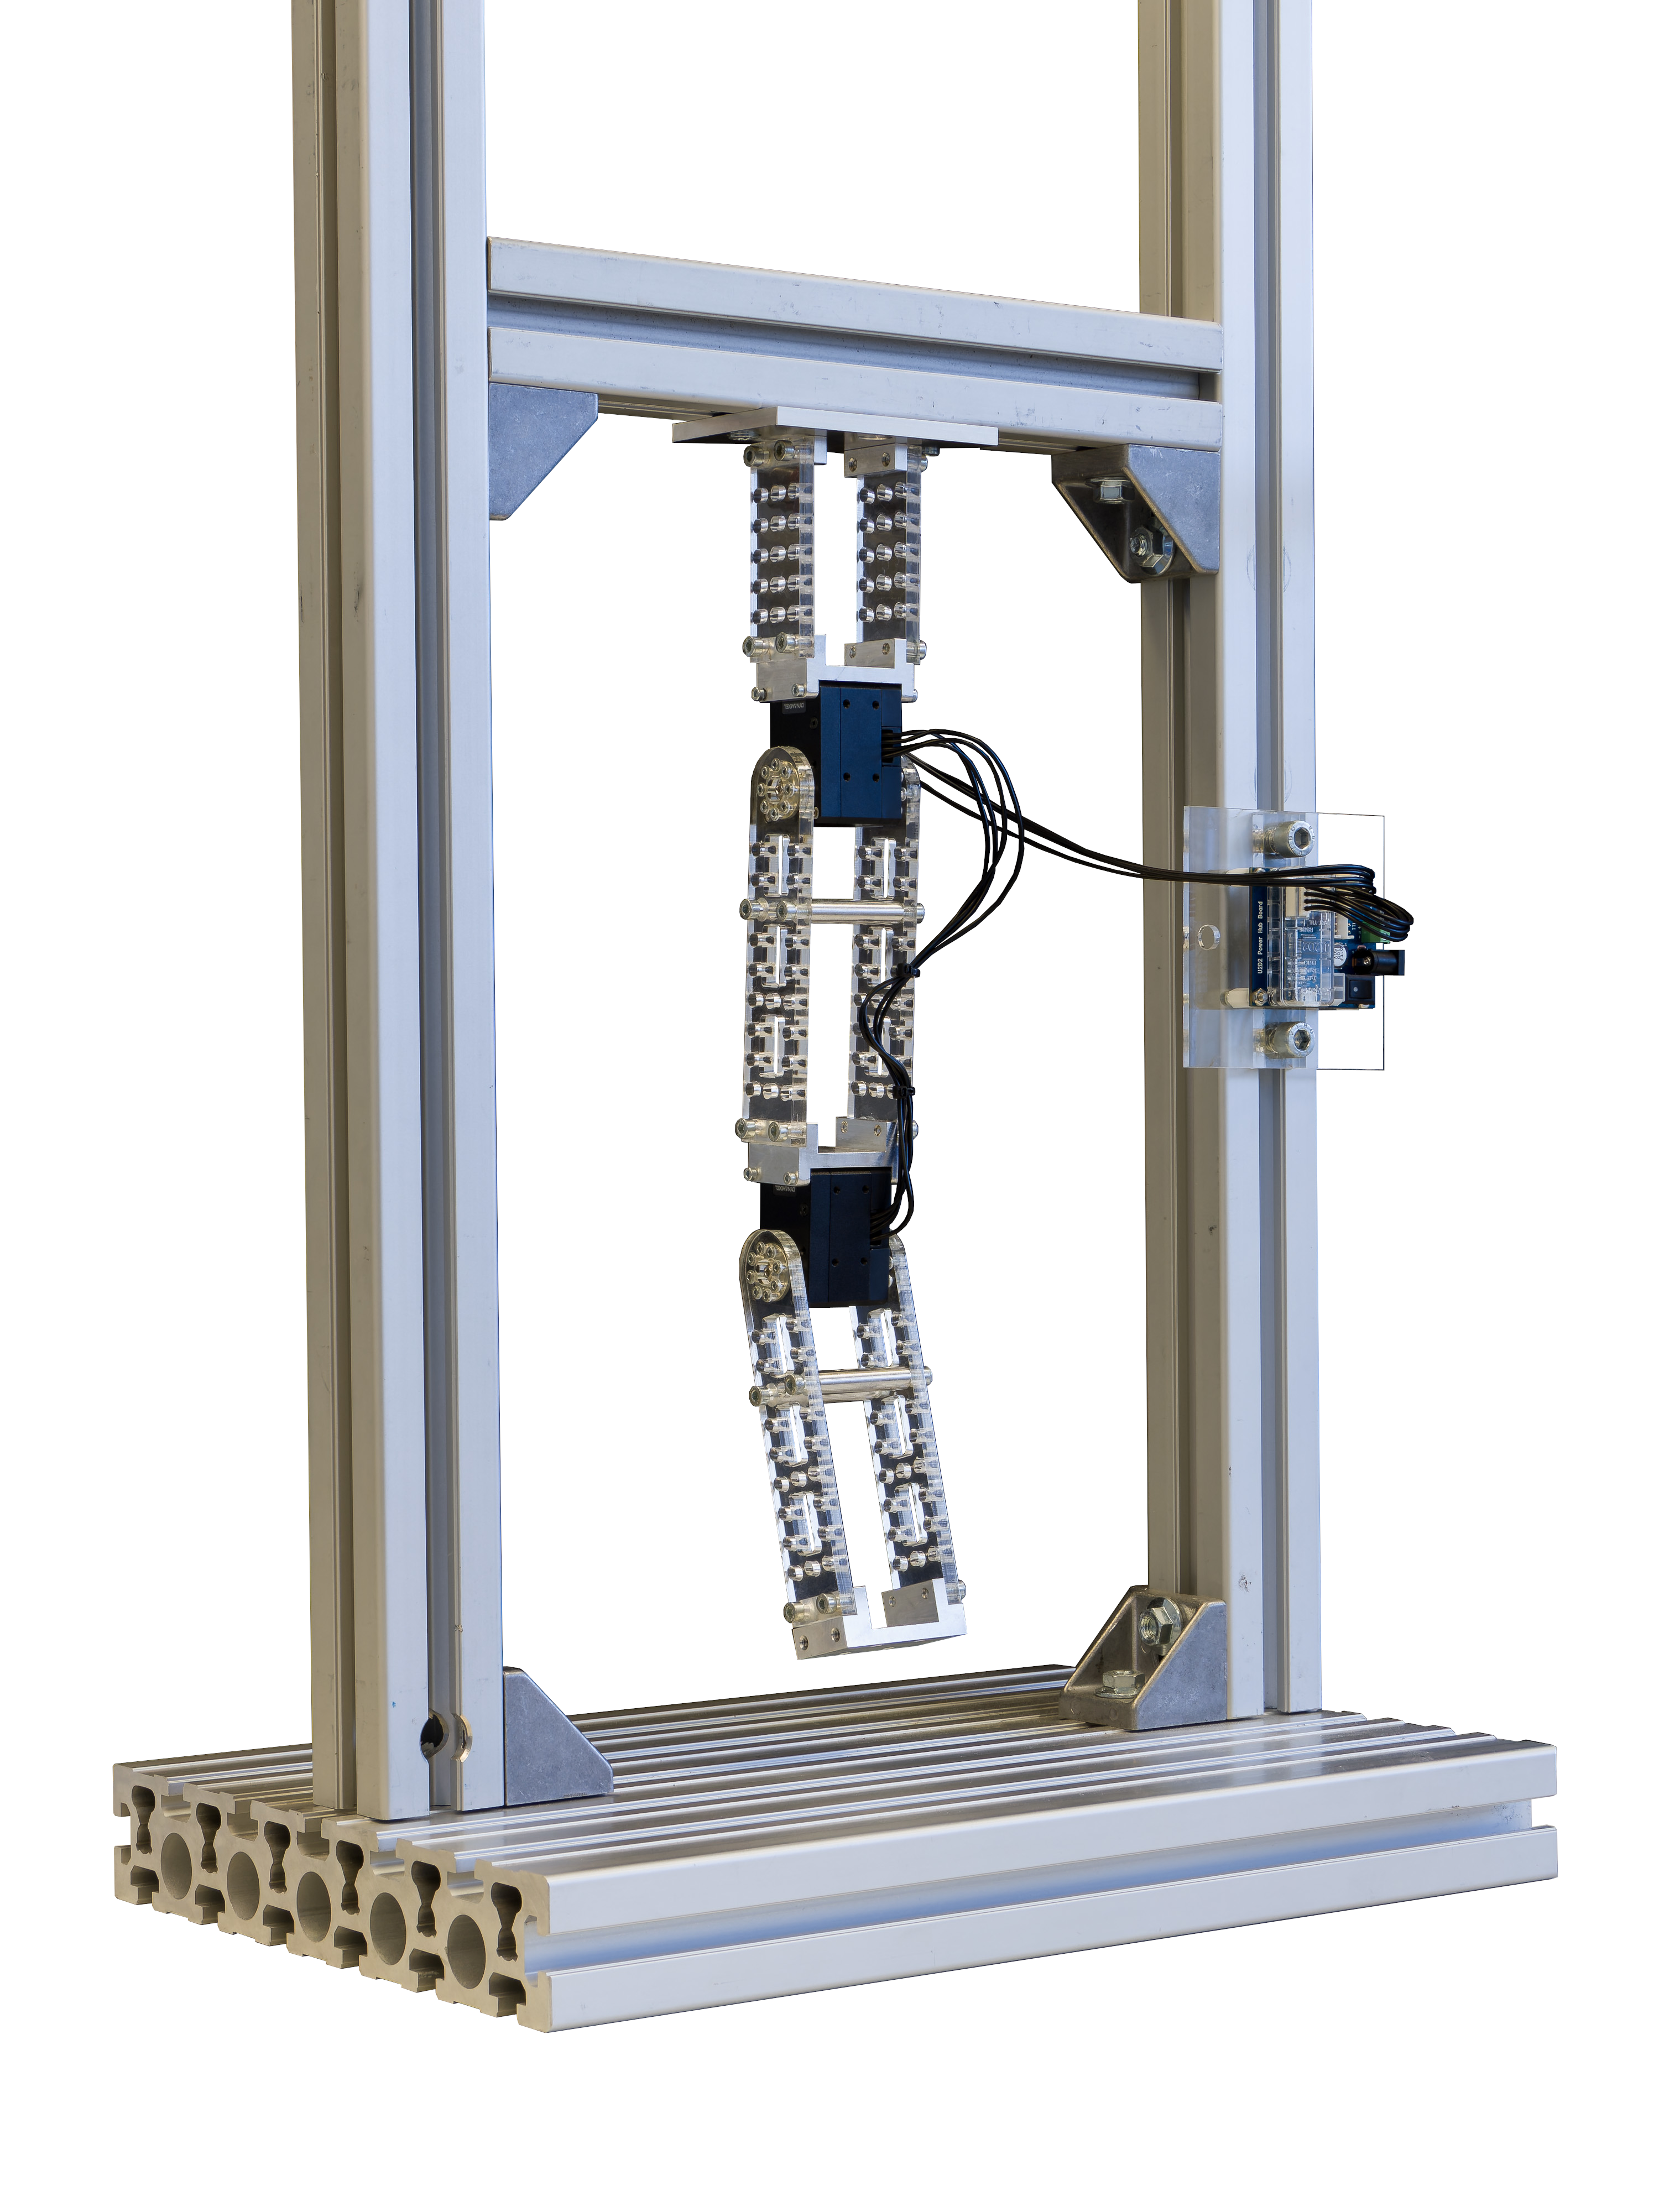
\includegraphics[height=7cm]{img/Versuchsaufbau.png}
	%	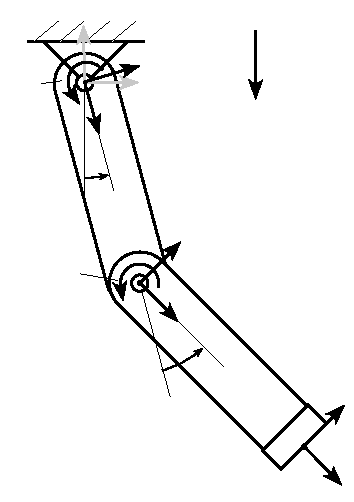
\includegraphics[height=7cm]{img/Zeichnung/Zeichnung.pdf}
	\hspace{1cm}
	\def\svgwidth{5.5cm}
	\input{img/Zeichnung/Zeichnung.pdf_tex}
	\caption{Foto sowie schematische Darstellung des zu untersuchenden Roboters~\cite{Fuchs23}.}
	\label{fig:Roboter}
\end{figure}

\def\myLineWidth{1.5pt}

% may define colors in advance, e.g., if they should be the same throughout the article
\definecolor{mycolor1}{cmyk}{100,70,0,0}%
\definecolor{mycolor2}{RGB}{255, 68, 76}% 
\begin{figure}[t]
	\centering
	% Minimal example for a TikZ plot

% 1) begin the overall picture
\begin{tikzpicture} 
    % 2) begin the axis
    \begin{axis}[%
        % 2a) define the properties of the axis
        width=\textwidth,   % width of the plot
        height= 5cm,       % height of the plot
        xmajorgrids,        % grid on
        xmin = -1,
        xmax = 11,
        ymajorgrids,
        ylabel={Auslenkung $\unit[y]{(m)}$},  % axis label (unit needs units-package)
        xlabel={Zeit $\unit[t]{(s)}$}
        ]
        
        % further may necessary setting:
%        xtick={0.5*pi, pi, 1.5*pi, 2*pi},   % modified xtick positions
%        xticklabels={$\pi/2$,$\pi$,$\nicefrac{3\pi}{2}$,$2\pi$},              % labels at previously set positions
%        ytick={-1,0,1},                 % analogous to x-ticks
%        yticklabels={-$\hat{y}$,0,$\hat{y}$}, 

%        ylabel={displacement $\unit[y]{(m)}$},  % axis label
%        % define legend
%        legend style={
%        	draw=black, % color of the border
%        	at={(0.5,1.05)}, % position plot has normalized wodth and length of 1
%        	anchor = south, % set legend at which anchor to defined position
%        	legend columns = 2, % legend entries in two columns
%        	/tikz/every even column/.append style={column sep=0.5cm} % space between legend's columns
%        }
%        ]
        
        
        % 2b) the plots itselves
        
        % insert data from txt-file
        \addplot[color = mycolor1, line width = \myLineWidth] table{img/plots/data/sin_data.txt}; % define plot properties in [...]
        \addlegendentry{$\sin$} % add legend entry

        \addplot[color = mycolor2, line width = \myLineWidth, dashdotted] table{img/plots/data/cos_data.txt}; % insert data from txt-file
        \addlegendentry{$\cos$} % add legend entry
        
        % manual plot
        \addplot[color = black, line width = 2.0, opacity = 0.5, forget plot] table[row sep=crcr] {%
        	%
        	-5	1\\
        	15 1\\
        }; 
    
    \end{axis}
    
\end{tikzpicture}%

	\caption{Beispielhafter Plot}
	\label{fig:plot_example}
\end{figure}

\bibliographystyle{itm_phd_deu}
\bibliography{literature.bib}

\end{document}